%!TEX program = xelatex
\documentclass[dvipsnames, svgnames,a4paper,11pt]{article}
% ----------------------------------------------------
%   中山大学物理与天文学院本科实验报告模板
%   作者:Huanyu Shi,2019级
%   知乎:https://www.zhihu.com/people/za-ran-zhu-fu-liu-xing
%   Github:https://github.com/Huanyu-Shi/SYSU-SPA-Labreport-Template
%   Last update : 2023.4.10
% ----------------------------------------------------

% ----------------------------------------------------- 
%	加边框的命令
%	参考:https://tex.stackexchange.com/questions/531559/how-to-add-the-page-border-for-first-two-pages-in-latex
\usepackage{tikz}
\usetikzlibrary{calc}
\usepackage{eso-pic}
\AddToShipoutPictureBG{%
\begin{tikzpicture}[overlay,remember picture]
\draw[line width=0.6pt] % 边框粗细
    ($ (current page.north west) + (0.6cm,-0.6cm) $)
    rectangle
    ($ (current page.south east) + (-0.6cm,0.6cm) $); % 边框位置
\end{tikzpicture}}


\usepackage{xcolor}
\definecolor{c1}{HTML}{2752C9} % 目录颜色
\definecolor{c2}{RGB}{190,20,83} % 引用颜色

\usepackage{ctex}
\usepackage[top=28mm,bottom=28mm,left=15mm,right=15mm]{geometry}
\usepackage{hyperref} 
\hypersetup{
	colorlinks,
	linktoc = section, % 超链接位置,选项有section, page, all
	linkcolor = c1, % linkcolor 目录颜色
	citecolor = c1  % citecolor 引用颜色
}
\usepackage{amsmath,enumerate,multirow,float}
\usepackage{tabularx}
\usepackage{tabu}
\usepackage{subfig}
\usepackage{fancyhdr}
\usepackage{graphicx}
\usepackage{wrapfig}  
\usepackage{physics}
\usepackage{appendix}
\usepackage{amsfonts}

%
\usepackage{tcolorbox}
\tcbuselibrary{skins,breakable}
\newtcolorbox{tbox}[2][]{
    colframe=black!70!,
    breakable,
    enhanced,
	boxrule =0.5pt,
    title = {#2},
    fonttitle = \large\kaishu\bfseries,
	drop fuzzy shadow,
    #1
}
\newtcolorbox[auto counter,number within=section]{question}[1][]{
  top=2pt,bottom=2pt,arc=1mm,
  boxrule=0.5pt,
%   frame hidden,
  breakable,
  enhanced, %跨页后不会显示下边框
  coltitle=c1!80!gray,
  colframe=c1,
  colback=c1!3!white,
  drop fuzzy shadow,
  title={思考题~\thetcbcounter:\quad},
  fonttitle=\bfseries,
  attach title to upper,
  #1
}
\newcommand{\setLhead}[1]{%
  \lhead{{\color{gray}\kaishu #1}} % 定义新的命令,设置右边页眉的内容
}
\newcommand{\setRhead}[1]{%
  \rhead{{\color{gray}\kaishu #1}} % 定义新的命令,设置右边页眉的内容
}
% ---------------------------------------------------------------------
%	利用cleveref改变引用格式,\cref是引用命令
\usepackage{cleveref}
\crefformat{figure}{#2{\textcolor{c2}{图 #1}}#3} % 图片的引用格式
\crefformat{equation}{#2{(\textcolor{c2}{#1})}#3} % 公式的引用格式
\crefformat{table}{#2{\textcolor{c2}{表 #1}}#3} % 表格的引用格式


% ---------------------------------------------------------------------
%	页眉页脚设置
\fancypagestyle{plain}{\pagestyle{fancy}}
\pagestyle{fancy}
\setLhead{中山大学物理与天文学院基础物理实验预习报告}
%\lhead{\kaishu 中山大学物理与天文学院物理实验\uppercase\expandafter{\romannumeral3}} % 左边页眉,学院 + 课程
%\rhead{{\color{gray}\kaishu Template 实验报告模板}} % 右边页眉,实验报告标题
\setRhead{实验1\hspace{1pt}冰的熔化热测量}
\cfoot{\thepage} % 页脚,中间添加页码


% ---------------------------------------------------------------------
%	对目录、章节标题的设置
\renewcommand{\contentsname}{\centerline{\huge 目录}}
\usepackage{titlesec}
\usepackage{titletoc}
% \titleformat{章节}[形状]{格式}{标题序号}{序号与标题间距}{标题前命令}[标题后命令]
\titleformat{\section}{\centering\LARGE\songti}{}{1em}{}

% ---------------------------------------------------------------------
%   listing代码环境设置
\usepackage{listings}
\lstloadlanguages{python}
\lstdefinestyle{pythonstyle}{
backgroundcolor=\color{gray!5},
language=python,
frameround=tftt,
frame=shadowbox, 
keepspaces=true,
breaklines,
columns=spaceflexible,                   
basicstyle=\ttfamily\small, % 基本文本设置,字体为teletype,大小为scriptsize
keywordstyle=[1]\color{c1}\bfseries, 
keywordstyle=[2]\color{Red!70!black},   
stringstyle=\color{Purple},       
showstringspaces=false,
commentstyle=\ttfamily\scriptsize\color{green!40!black},%注释文本设置,字体为sf,大小为smaller
tabsize=2,
morekeywords={as},
morekeywords=[2]{np, plt, sp},
numbers=left, % 代码行数
numberstyle=\it\tiny\color{gray}, % 代码行数的数字字体设置
stepnumber=1,
rulesepcolor=\color{gray!30!white}
}




% ---------------------------------------------------------------------
%	其他设置
\def\degree{${}^{\circ}$} % 角度
\graphicspath{{./images/}} % 插入图片的相对路径
\allowdisplaybreaks[4]  %允许公式跨页 % 导入模板的相关设置
\usepackage{lipsum}
\usepackage{indentfirst}
\usepackage{pdfpages}
\usepackage{multirow}
\usepackage{subfig}
\usepackage{graphicx}
\usepackage{float} 
\renewcommand{\d}{\mathrm{d}}


%---------------------------------------------------------------------
%	正文
%---------------------------------------------------------------------
\setRhead{磁滞回线的测量}%实验名称
\begin{document}


\begin{table}
	\renewcommand\arraystretch{1.7}
	\begin{tabularx}{\textwidth}{
		|X|X|X|X
		|X|X|X|X|}
	\hline
	\multicolumn{2}{|c|}{预习报告}&\multicolumn{2}{|c|}{实验记录}&\multicolumn{2}{|c|}{分析讨论}&\multicolumn{2}{|c|}{总成绩}\\
	\hline
	 25& &30  & &25  & &80& \\
	\hline
	\end{tabularx}
\end{table}


\begin{table}
	\renewcommand\arraystretch{1.7}
	\begin{tabularx}{\textwidth}{|X|X|X|X|}
	\hline
	年级专业:& 2023级物理学类 &组号& 1\\
	\hline
	姓名:& 姚昊廷  & 学号:&22322091\\
	\hline
	日期:& 2024.10.17& 教师签名:& \\
	\hline
	\end{tabularx}
\end{table}

\begin{center}
	\LARGE 磁滞回线的测量
\end{center}

\textbf{【实验报告注意事项】}
\begin{enumerate}
	\item 实验报告由三部分组成:
	\begin{enumerate}
		\item 预习报告:(提前一周)认真研读\underline{\textbf{实验讲义}},弄清实验原理;实验所需的仪器设备、用具及其使用(强烈建议到实验室预习),完成课前预习思考题;了解实验需要测量的物理量,并根据要求提前准备实验记录表格(第一循环实验已由教师提供模板,可以打印)。预习成绩低于10分(共20分)者不能做实验。
	    \item 实验记录:认真、客观记录实验条件、实验过程中的现象以及数据。实验记录请用珠笔或者钢笔书写并签名(\textcolor{red}{\textbf{用铅笔记录的被认为无效}})。\textcolor{red}{\textbf{保持原始记录,包括写错删除部分,如因误记需要修改记录,必须按规范修改。}}(不得输入电脑打印,但可扫描手记后打印扫描件);离开前请实验教师检查记录并签名。
	    \item 分析讨论:处理实验原始数据(学习仪器使用类型的实验除外),对数据的可靠性和合理性进行分析;按规范呈现数据和结果(图、表),包括数据、图表按顺序编号及其引用;分析物理现象(含回答实验思考题,写出问题思考过程,必要时按规范引用数据);最后得出结论。
	\end{enumerate}
	\textbf{实验报告就是将预习报告、实验记录、和数据处理与分析合起来,加上本页封面。}
	\item 每次完成实验后的一周内交\textbf{实验报告}(特殊情况不能超过两周)。
	\item 除实验记录外,实验报告其他部分建议双面打印。
\end{enumerate}

{\textbf{【注意事项】}
\begin{enumerate}
	\item 注意用电安全,电源电压和电流按要求设置;
	\item 如发现线圈或者电阻过热,要及时关闭电源,避免烫伤;
	\item 实验中,要求采样电阻两端电压幅值不能超过±1V;
    \item 注意myDAQ数据采集单元的输入电压不能超过±10V,应在±6V以内;
    \item 为防止仪器损坏,调整电路时应关闭电源,其他疑难故障请询问老师;
    \item 得到测量结果后,应及时点击输出开关,关闭电源,防止电阻长时间使用而发烫,甚至损坏。
    
\end{enumerate}}

\clearpage
\tableofcontents
\clearpage

\setcounter{section}{0}
\section{磁滞回线的测量}
	
\subsection{实验目的}
\begin{enumerate}
	\item 加深对铁磁材料的磁化曲线、磁滞回线、剩磁、矫顽力等物理概念的理解;
	\item 用数值积分法测量磁感应强度,从而测量磁滞回线。
\end{enumerate}

\subsection{仪器用具}
\begin{table}[htbp]
	\centering
	\renewcommand\arraystretch{1.6}
	% \setlength{\tabcolsep}{10mm}
	\begin{tabular}{p{0.05\textwidth}|p{0.20\textwidth}|p{0.05\textwidth}|p{0.5\textwidth}}
	\hline
	编号& 仪器用具名称 & 数量 &  主要参数(型号,测量范围,测量精度等) \\
	\hline
	1&电源&1 &\\
	\hline
	2&功率放大电路板 &1&\\
	\hline
	3&环形变压器 & 1 &硅钢材料 \\
	\hline
	4&碳钢材料铁芯&1 &  \\
	\hline
	5& 坡莫合金铁芯&1& \\
	\hline
	6& myDAQ数据采集单元&1& \\
	\hline
	7& 实验电路板&1& \\
	\hline
	8& 导线&若干& \\
	\hline
\end{tabular}
\end{table}

\textbf{原理概述}
\section*{1. 铁磁材料的磁滞现象}
对已退磁的铁磁材料(材料内部磁化强度 $M=0$ )施加磁场时,材料会被磁化(如图1所示), 磁化开始时, 磁感应强度 $B$ 随磁场强度 $H$ 的增加而增加, 即曲线 $0 a$ 段,称为起始磁化曲线。当 $H$ 增加到一定值后, $B$ 的增加趋于缓慢,磁化强度 $M$ 在 $a$ 点后达到饱和(如图1左图),即 $M$ 不再随磁场强度增加而增加;此时对应磁感应强度 $B=$ $\mu_{0}(H+M)$ 变化缓慢(对铁磁材料, $M \gg H$ 或相对磁导率 $\mu_{r} \gg 1$ ),我们称 $a$ 点对应磁化强度 $M_{S}$ 称为饱和磁化强度,相应地,对应的 $H_{S}$ 称为饱和磁场强度、 $B_{S}$ 称为饱和磁感应强度(如图1右图)。此时如果将 $H$ 由饱和点加大到 $H_{m}$ 并退回,磁化曲线是可逆的、重合的。当外加 $H$ 由 $H_{s}$ 变到 $-H_{s}$ ,再由- $H_{s}$ 变到 $H_{s}, M$ 或 $B$ 将随 $H$ 的变化而变化,形成一条对称的闭合曲线(即 $a \rightarrow b \rightarrow c \rightarrow d \rightarrow e \rightarrow f \rightarrow a$ ),称为该铁磁材料的磁滞回线。

从图1可以看出, $\underline{B}$ 的变化总是落后于 $H$ 的变化,当 $H=0$ 时, $M$ 和 $B$ 不为零,这个量就是铁磁材料的"剩磁",大小分别为 $M_{r}$ 和 $B_{\mathrm{r}}$ ,分别称为剩余磁化强度和剩余磁感应强度。如果想使 $B$ (或 $M$ )变为零,则必须加一反向磁场 $H_{c}, H_{c}$ 即为铁磁材料的"矫顽力"。矫顽力大的称为硬磁材料,反之称为软磁材料。如果将铁磁材料置于周期性变化的磁场中, 它将被反复磁化, 由此得到的磁滞回线称为动态磁滞回线(Dynamic Magnetization Curve)。\\



如果由小到大选取不同的最大磁场强度 $H_{\mathrm{m}}$, 则可得到一系列由小到大的磁滞回线,如图2 所示。这些曲线的顶点连接起来( $\left.0 \rightarrow a_{1} \rightarrow a_{2} \rightarrow a_{3} \rightarrow a\right)$ ,得到的 $B-H$ 曲线称为铁磁材料的基本磁化曲线。通常该曲线与其起始磁化曲线并不一定完全重合。

铁磁材料的另一个重要磁性参数是铁芯的磁滞损耗 $W e$ 。所谓铁芯损耗是指单位体积铁磁材料交流磁化一周损耗的能量,即

$$
\Delta W=\oint B d H
$$

即动态磁滞回线所围的面积(思考变压器中使用的线圈缠绕的磁芯材料选择有何考量)。\\
铁磁材料在磁化过程中有剩磁存在,表明磁化过程的不可逆性。对于已经磁化了的铁磁材料, 简单地加个反向磁场, 并不能使之退磁。如欲退磁, 可将其置于线圈中,首先在线圈中通以大电流,使磁铁达到磁饱和状态。然后,减小电流,使磁铁继续达到新的饱和状态。重复此过程,直至电流减小为接近零。在这个操作过程中,可检测出一连串逐渐缩小的、最终趋向原点的不封闭曲线,如图3所示,就达到了退磁的目的。用交流电退磁时,因电流方向自动改变,故只需逐渐减小电流大小即可。\\



\section*{2. 磁滞回线测量原理}


图4 基于 myDAQ 测量数值积分法的磁滞回线测量电路原理图\\
图 4 为基于 myDAQ 数据采集通过数值积分描绘磁滞回线的原理电路图,对于我们的实验仪器,互感线圈的初级匝数 $N_{1}$ 和次级匝数 $N_{2}$ 在 0-400 匝(共 6 个抽线头);通过一体机电脑上的软件控制 myDAQ 模块的模拟输出端口,输出指定频率、幅值和偏置量的交流信号,该交流信号经过功率放大模块后,作为初级线圈的输入激励信号( $\tilde{I}_{1}$ );电流采样电阻 $R_{1}$ 为功率电阻, 阻值可任选。

当绕在环形铁磁芯的初级线圈 $N_{1}$ 通过交变电流 $\tilde{I}_{1}$ 时, 根据安培环路定理, 在环形铁芯内产生的磁场强度 $\widetilde{H}$ 为


\begin{equation*}
\widetilde{H}=\frac{N_{1}}{l} \tilde{I}_{1} \tag{1}
\end{equation*}


在无漏磁的理想情况下,由法拉第电磁感应定律得,在次级线圈 $N_{2}$ 中产生的交变电动势 $\tilde{e}_{2}$ 为


\begin{equation*}
\tilde{e}_{2}=-N_{2} \frac{d \Phi}{d t}=-N_{2} A \frac{d \tilde{B}}{d t} \tag{2}
\end{equation*}


式中, $N_{1}$ 为初级线圈的匝数, $l$ 为环形铁芯的平均磁路长度; $N_{2}$ 为次级线圈的币数, $A$为环形铁芯的截面积。

与初级线圈串联的电阻 $R_{1}$ 为取样电阻。将 $R_{1}$ 上的电压 $\widetilde{U}_{1}$ 接到数据采集单元测量,则


\begin{equation*}
\widetilde{H}=\frac{N_{1}}{l} \cdot \frac{\widetilde{U}_{1}}{R_{1}} \tag{3}
\end{equation*}


由于 $N_{1} 、 l 、 R_{1}$ 皆为已知不变量,所以数据采集单元测量的电压 $\widetilde{U}_{1}$ 就与磁场强度 $\widetilde{H}$的大小成正比。铁磁材料内部磁感应强度由式(2)积分


\begin{equation*}
\tilde{B}(t)=-\int_{0}^{t} \frac{\tilde{e}_{2}(t)}{N_{2} A} d t \tag{4}
\end{equation*}


采用数值积分方法 (如图4所示), 设初级线圈电流由函数发生器提供:


\begin{equation*}
\tilde{I}_{1}(\omega)=G(\omega) U_{0} \cos \left(\omega t+\theta_{I}\right)=U_{1} \cos \left(\omega t+\theta_{I}\right) / R_{1} \tag{5}
\end{equation*}


$U_{0} \cos (\omega t)$ 为函数发生器的输出电压, $\theta_{I}$ 为互感器初级线圈电流相对于函数发生器输出电压的相位差, $G(\omega)$ 为初级线圈及其电流取样电阻组成电路的电导,它与频率成反比, 因此, 频率越高, 电流越低。 $\tilde{I}_{1}$ 可直接从初级线圈电流取样电阻 $R_{1}$ 中获取 $\tilde{I}_{1}=$ $\widetilde{U}_{1} / R_{1}$ 。

次级线圈的输出电压直接接入 myDAQ 的输入端, 其输入电阻 $\left(10 \mathrm{G} \Omega\right.$, 即 $1 \times 10^{10} \Omega$,加保护电阻 $100 \mathrm{k} \Omega$ )远高于次级线圈组的最大输出阻抗,该输出电压信号可视为等于输出电动势。


\begin{equation*}
\tilde{e}_{2} \cong U_{2}=U_{2} \cos \left(\omega \mathrm{t}+\theta_{V}\right) \tag{6}
\end{equation*}


从式(4)可知,对 myDAQ 的 Y 端输入采样进行数值积分便可获得磁感应强度 $B$ 。结合公式(3)得到的磁场 $H$ ,在所使用的 Labview 数据采集软件中作图得到磁滞回线。

\subsection{实验前思考题}
\begin{question}
	对于铁磁性物质,为什么缠上线圈,通上电流,就能在缠绕物质中产生非常强的磁感应强度?微观物理机制是什么?
	\tcblower
	铁磁性物质在缠绕线圈中通电后能够产生强大的磁感应强度的原因主要与以下几个方面有关:
	\begin{enumerate}
		\item 自旋与磁矩:铁磁性材料中的原子具有自旋,导致它们产生磁矩。在铁磁性材料中,原子的磁矩会自发地取向,形成宏观的磁性。
		\item 对齐机制:当外部电流通过线圈时,线圈产生的磁场会影响铁磁性材料中的原子。电流产生的磁场会与材料内部的原子磁矩相互作用,使得这些磁矩趋向于与外部磁场对齐。由于铁磁性材料中存在强的交换作用力,原子间的磁矩可以保持一致的方向。
		\item 磁场增强:通电线圈产生的磁场在铁磁性材料内部被增强,主要是因为材料的高磁导率。铁磁性材料的磁导率远高于空气或真空,使得在其内部,磁场的强度大幅提升。
		\item 饱和磁性:当外部磁场增强到一定程度时,铁磁性材料中的磁矩几乎全部对齐,这被称为饱和状态。在饱和状态下,磁感应强度达到最大值,且几乎不再随外部磁场的增加而增加。
		\item 滞后现象:铁磁材料的磁性不仅与当前的外部磁场有关,还与其过去经历的磁场有关。这种特性会导致磁性材料在去除外部磁场后仍然保持一定的磁感应强度。
	\end{enumerate}
总体来看,铁磁性材料能够在电流通过的线圈中产生强磁感应强度的微观机制涉及到原子的自旋和磁矩对齐、材料的高磁导率、以及材料的饱和和滞后特性。通过这些微观机制,外部电流产生的磁场能在铁磁性材料中得到有效的放大。
\end{question}

\begin{question}
	如何选择初级线圈的匝数,次级线圈匝数,电流采样电阻$R_1$?如何设置交流电压频率和电压幅值,两者间有何关系,如何避免线圈中电流过大?
	\tcblower
	$N_1$取400,线圈密度一定时,越长(匝数越多)就越接近“无限长线圈”的模型,即可以忽略掉边界效应,由安培环路定理
	近似得到的$H=\frac{N_1}{l}I_1$就越接近真实值。
	$N_2$取100,次级线圈作为测量“铁磁性物质$B$关于$H$的滞后性”的设备应尽可能减少对铁磁质的干扰,$I_2N_2$尽可能下,故$N_2$
	取较小值。
	$R_1$可取1$\Omega$(最小)获得相同电流时功率小,发热少,在只考虑电阻阻值被温度影响时误差更小。且$R_1$较小可以
	使得电压表测得的电压更准确。
	$f$应在多次测量中取得合适值。$f$太高会使得$U$的电压集中在$L'$上导致$I_1$电流太小;$f$太小会导致$\varepsilon_2=\frac{\d \Phi}{\d t}$太小
	不便于测量,且数值积分法的积累误差会随所需时间上升而上升。
	电压峰值应灵活下调,通过调节电压峰值应测出同一种材料的基本磁化曲线、磁滞回线、退磁曲线等。
	下调$f$时,应保证$U$在较低水平,即$I_1$不接近$I_1$的上限。因为$U$固定时$U_R\propto I_1$随$f$减小而增大。
\end{question}



\clearpage
\setLhead{中山大学物理与天文学院基础物理实验记录}
\begin{table}
	\renewcommand\arraystretch{1.7}
	\centering
	\begin{tabularx}{\textwidth}{|X|X|X|X|}
	\hline
	专业:& 物理学类 &年级:& 2023级 \\
	\hline
	姓名:& 姚昊廷 &学号:&22322091  \\
	\hline
	室温:&25.0$^\circ$C&实验地点:&A507\ A4\\
	\hline
	学生签名:& & 评分: &\\
	\hline
	实验时间:& 2024.10.17& 教师签名:&\\
	\hline
	\end{tabularx}
\end{table}

\section{磁滞回线的测量}
\textbf{【实验内容、步骤、结果】}(按照实验内容和步骤依次简要记录每项实验的“内容、步骤、结果”,注意包含实验数据、现象照片或现象描述等)

一、实验内容

(1)测试环形变压器(硅钢材料)在三组不同频率和幅值激励信号下的饱和磁滞回线,给出剩磁、矫顽力、饱和磁滞回线所围面积、相对磁导率曲线;

(2)选择其中一组频率和幅值激励信号,分别测试坡莫合金和碳钢材料的磁滞回线,与相应的环形变压器的磁滞回线进行对比,观察和分析这三种材料磁滞回线的差异。

二、实验步骤

\begin{enumerate}
	\item 连接电路并沿信号检查电路;
	\item 开启电源并点击软件内启动按钮和记录按钮;
	\item 调整幅值和频率直到出现完整磁滞回线;
	\item 更换铁芯材料重复上述操作。
\end{enumerate}

三、实验结果
\begin{figure}[htbp]
	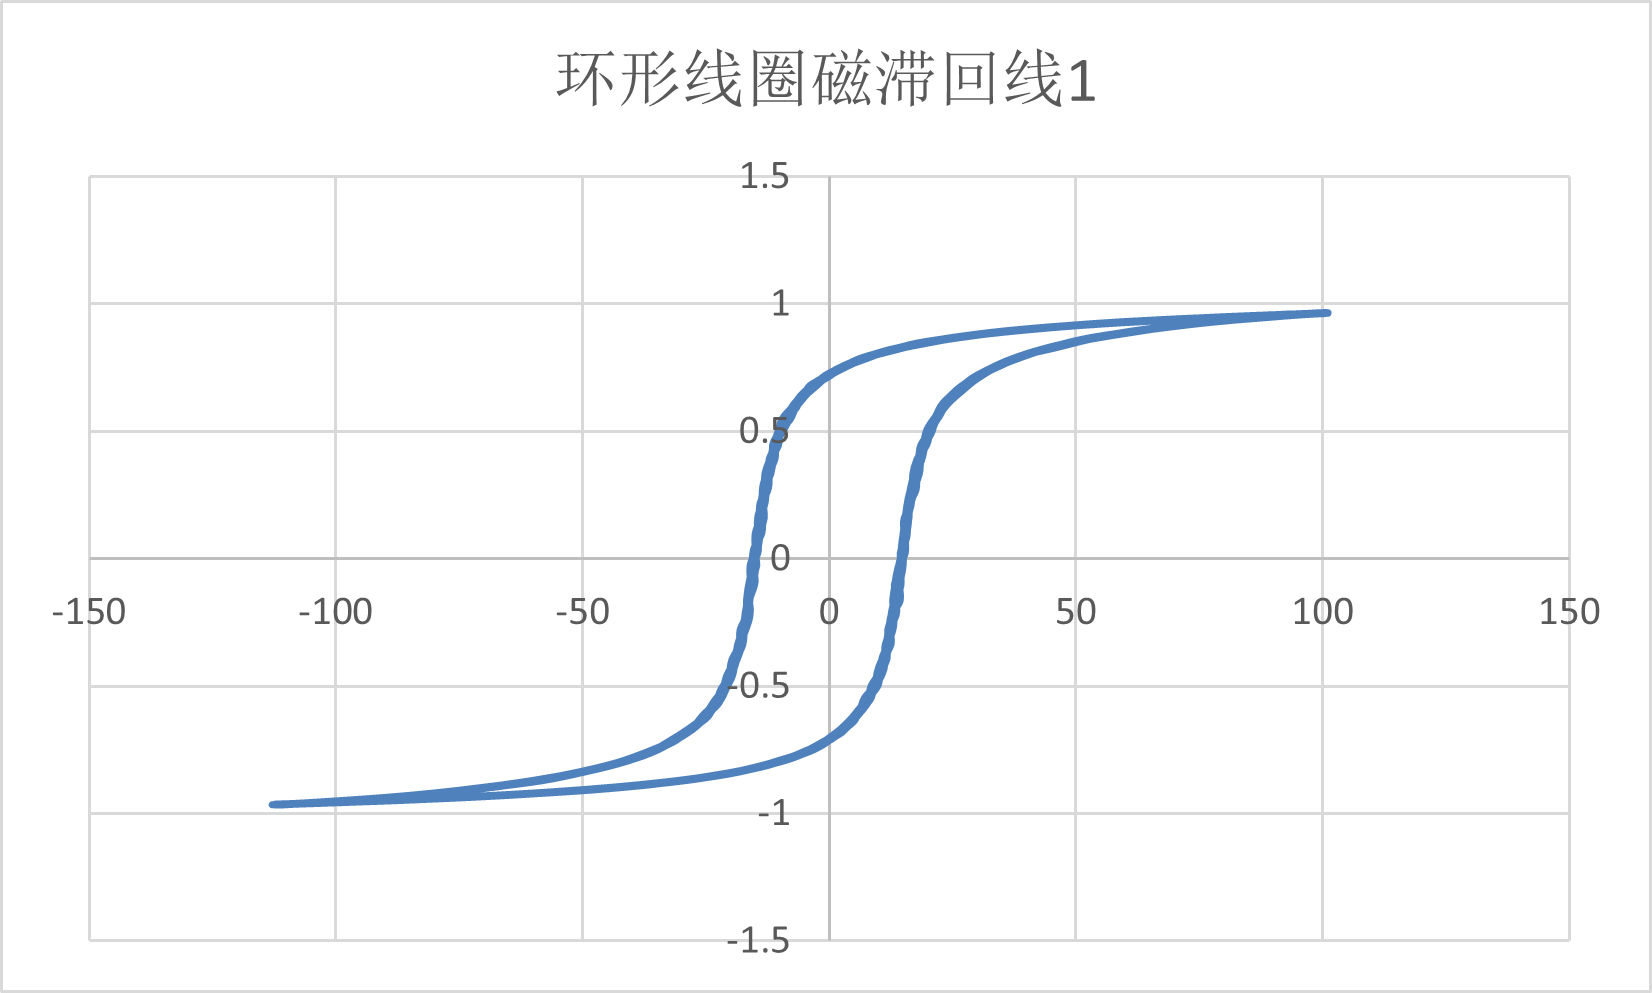
\includegraphics{磁滞回线/图片1.png}
\end{figure}
\begin{figure}[htbp]
	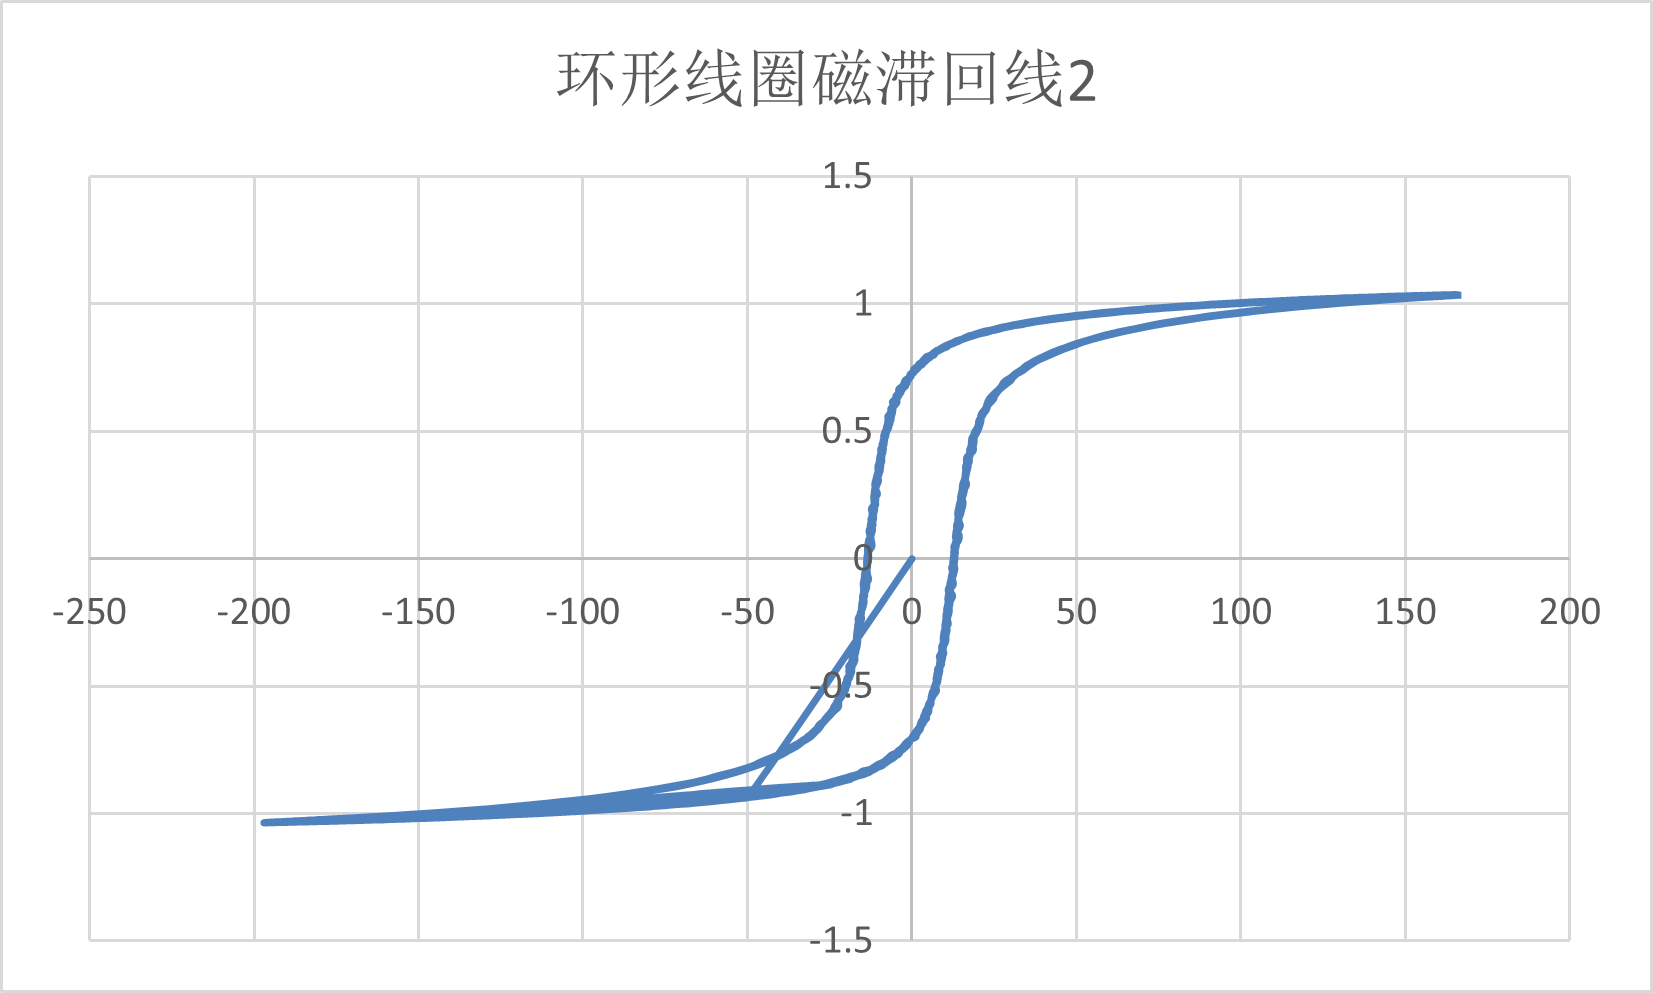
\includegraphics{磁滞回线/图片2.png}
\end{figure}
\begin{figure}[htbp]
	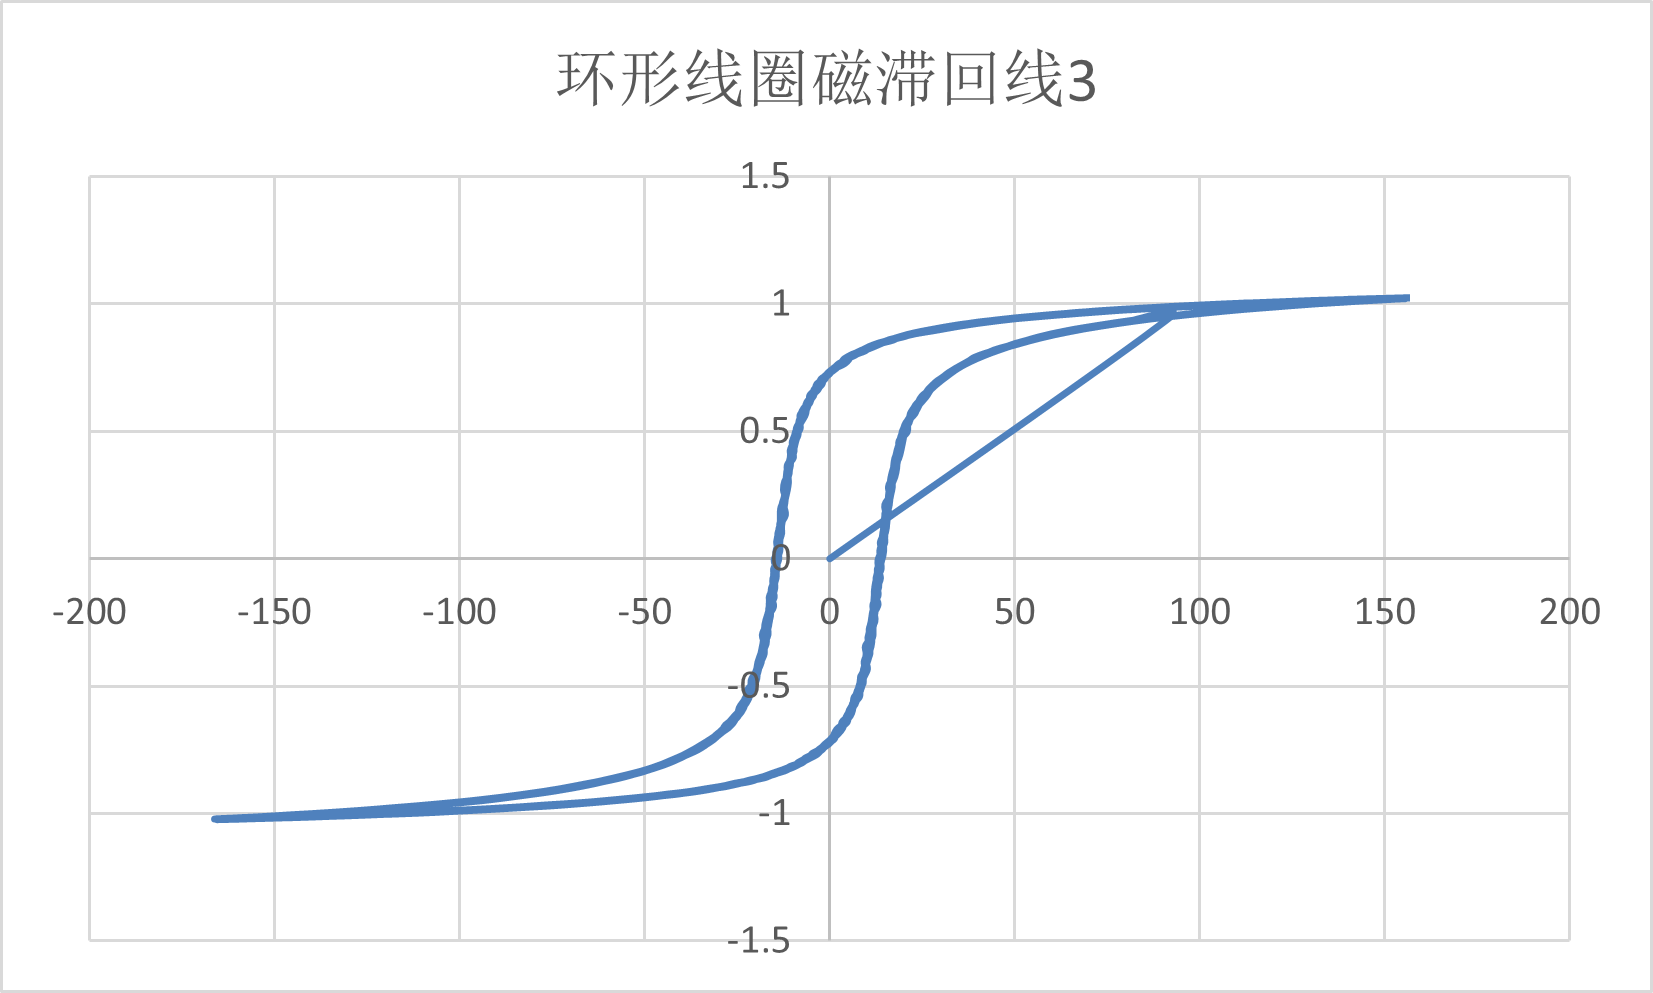
\includegraphics{磁滞回线/图片3.png}
\end{figure}
\begin{figure}[htbp]
	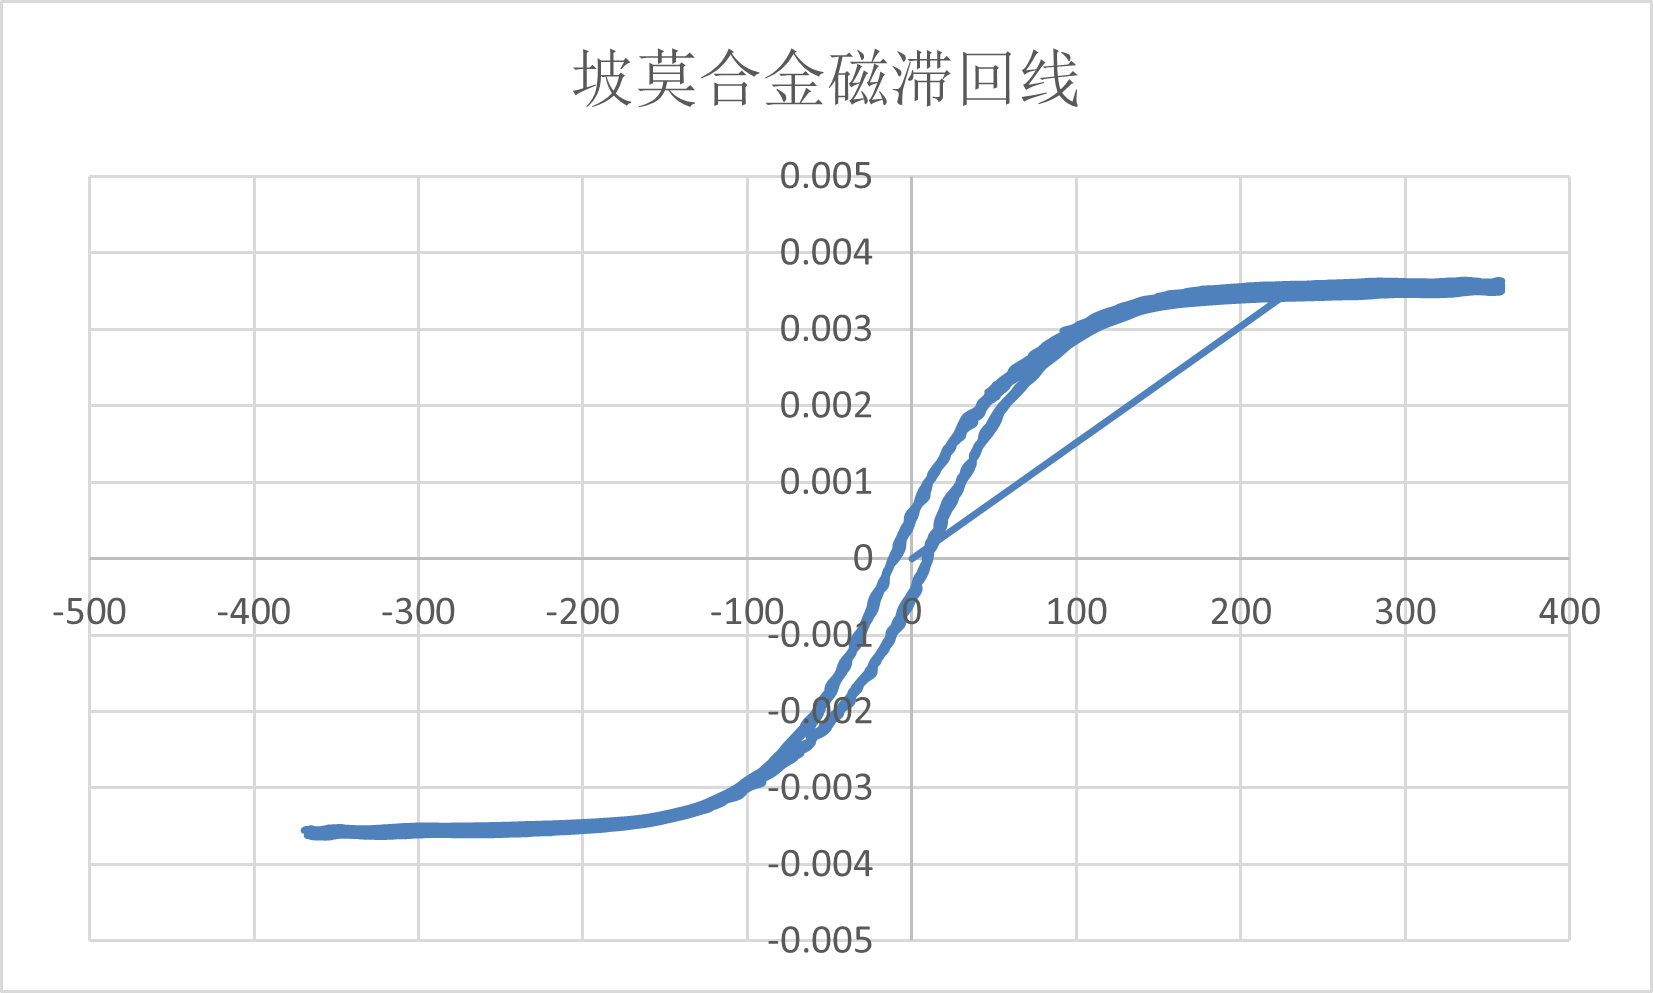
\includegraphics{磁滞回线/图片4.png}
\end{figure}
\begin{figure}[htbp]
	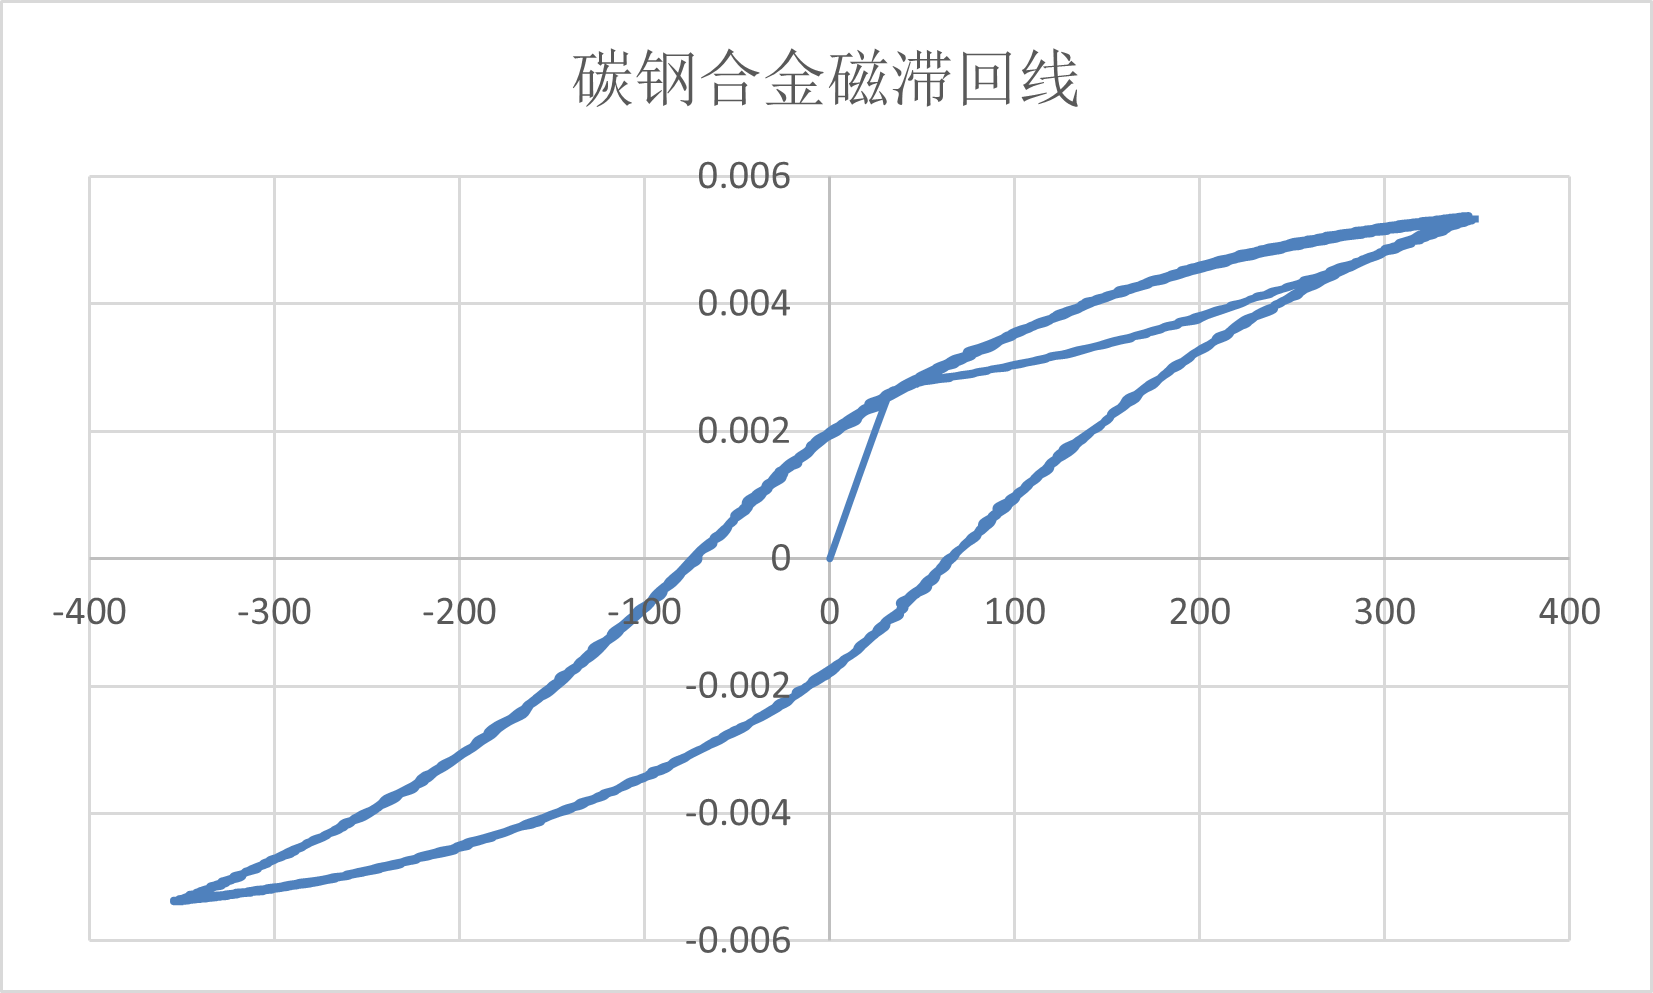
\includegraphics{磁滞回线/图片5.png}
\end{figure}
\section{各种导出量计算}
\textbf{剩余磁化强度:}$M_r=\frac{B_r}{\mu_0}=2.98\times10^6$V/m\\
\textbf{矫顽力:}$H_c=6.75$V/m\\
\textbf{最大磁能面积:}$\oint B\d H=15.3\text{J/m}^3$

\begin{figure}[htbp]
	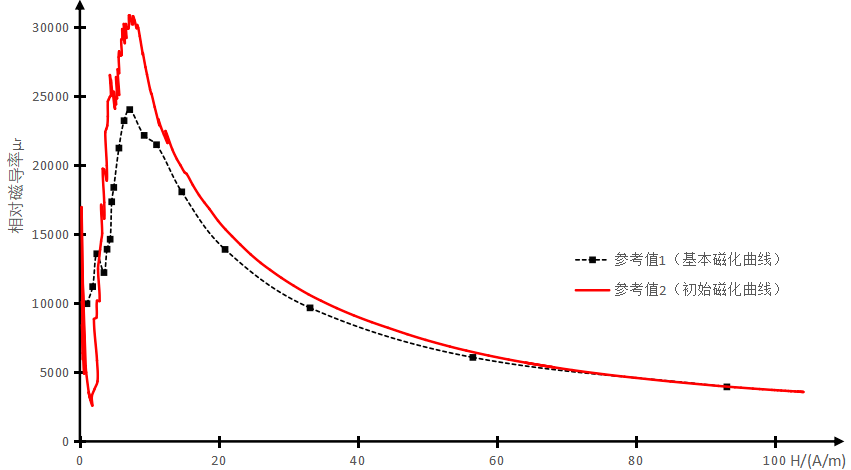
\includegraphics{磁滞回线/图片6.png}
	\caption{$\mu_r-H$曲线}
\end{figure}
\newpage


\subsection{实验过程中遇到的问题记录}



\clearpage
\setLhead{中山大学物理与天文学院基础物理实验分析与讨论}
\begin{table}
	\renewcommand\arraystretch{1.7}
	\begin{tabularx}{\textwidth}{|X|X|X|X|}
	\hline
	专业:& 物理学 &年级:& 2023级\\
	\hline
	姓名: &姚昊廷 & 学号:& 22322091\\
	\hline
    日期:&2024.10.17 & 评分: &\\
	\hline
	\end{tabularx}
\end{table}

\section{磁滞回线的测量}

\textbf{【分析与讨论】}

{\begin{center}
	\textbf{误差分析}
\end{center}}

本实验主要误差由线圈形状引起,因为现实中并不存在无限长线圈,故导致公式
$$H=\frac{N_1V_1}{lR_1}$$
并不准确。旧的方形线圈粗细非常不均(铁芯处的横截面为$64mm^2$,而最细处只有$24mm^2$),由于磁
场是“无源场”,那么无磁漏和磁路中心线上磁场大小处处相等(起码不能有太大差别)的假设
无法同时成立。另外,若假设无磁漏,则截面积不同之处$H$ 的值也会相差很大,这就导致整块
材料磁化非常不均。所以最后所得的$B−H$ 关系就非常不准确,存在非常大的误差。由于这项
巨大的误差,其他的例如仪器B 类误差、统计误差、舍入误差等都基本没有分析的意义。
新线圈的形状就能几乎完美地避免了这个问题。
另外,旧的方形线圈在测量横截面积$A$ 和平均磁路长度$l$ 时,我们也遇到了不小的麻烦。我
们在此不累述,新线圈的形状在估计$l$ 时情况就较为容易了。显然$A$ 是常数,可以用$D_1$,$D_2$, $h$
接计算。其中$l=\frac{\pi(D_1+D_2)}{2}$给出的计算方法既符合我们的几何直觉,又能满足$V = Al$ 的关系式,便
于直接用“每周期单位体积的磁滞损耗”计算总磁滞损耗,我们因此认为$l=\frac{\pi(D_1+D_2)}{2}$ 非常理想。

\textbf{【实验后思考题】}
\begin{question}
	各向异性磁电阻(AMR) 传感器为何要退磁?
	\tcblower
	AMR 中的磁簧片是铁磁性体,如果未退磁就继续使用,会导致在检测磁场方向上(两个
相反的方向),两个相反方向的最小触发电路切换的磁场强度不一致,其一比预设值小,另一比
预设值大。只有退磁后使用才能保证两个相反方向的最小触发值理论上相等。
\end{question}

\begin{question}
	为什么输入、输出正弦波会发生畸变?什么情况下畸变比较小?
	\tcblower
	若$B-H$ 关系是线性的,则次级线圈的电流相对初级线圈,应有$\frac{\pi}{2}$的相位滞后;次级线
圈产生的磁场反作用于初级线圈,产生再滞后$\frac{\pi}{2}$
相位的电动势。两次滞后总共滞后$\pi$相位,只
会削弱初级线圈的信号,并不会使初级线圈电流的正弦波畸变。(互感)
若$B-H$ 关系是非线性的,次级线圈的感应电流可能不再是正弦波,两次“相位”滞后也
不一定都是$\frac{\pi}{2}$
,从而使输入、输出信号可能都发生畸变。简而言之,就是磁滞现象。
材料接近退磁状态并且H 较小时,或使用磁能积较小的材料时,畸变较小。
\end{question}

\begin{question}
	铁磁材料的磁导率在什么条件下才可以近似为一常数?
	\tcblower
	材料接近退磁状态,且磁感应强度远小于饱和磁感应强度时。
\end{question}
\clearpage
% ---------------------------------------------------------------------
%   参考文献
%   注:使用参考文献时应按照xelatex->bibtex->xelatex->xelatex顺序进行编译
\phantomsection
%\addcontentsline{toc}{section}{参考文献}
\bibliographystyle{unsrt}
\bibliography{myref}
%\begin{thebibliography}{9}
	%\bibitem{ref1} 凤飞龙,黄育红,金蔚,王公正,崔致远,“外推法计算冰的熔解热的理论依据及Matlab实现方案”,《大学物理》,第42卷,第2期
%\end{thebibliography}


\clearpage
\appendix
\appendixpage
\addappheadtotoc
%\subsection*{相图代码}
%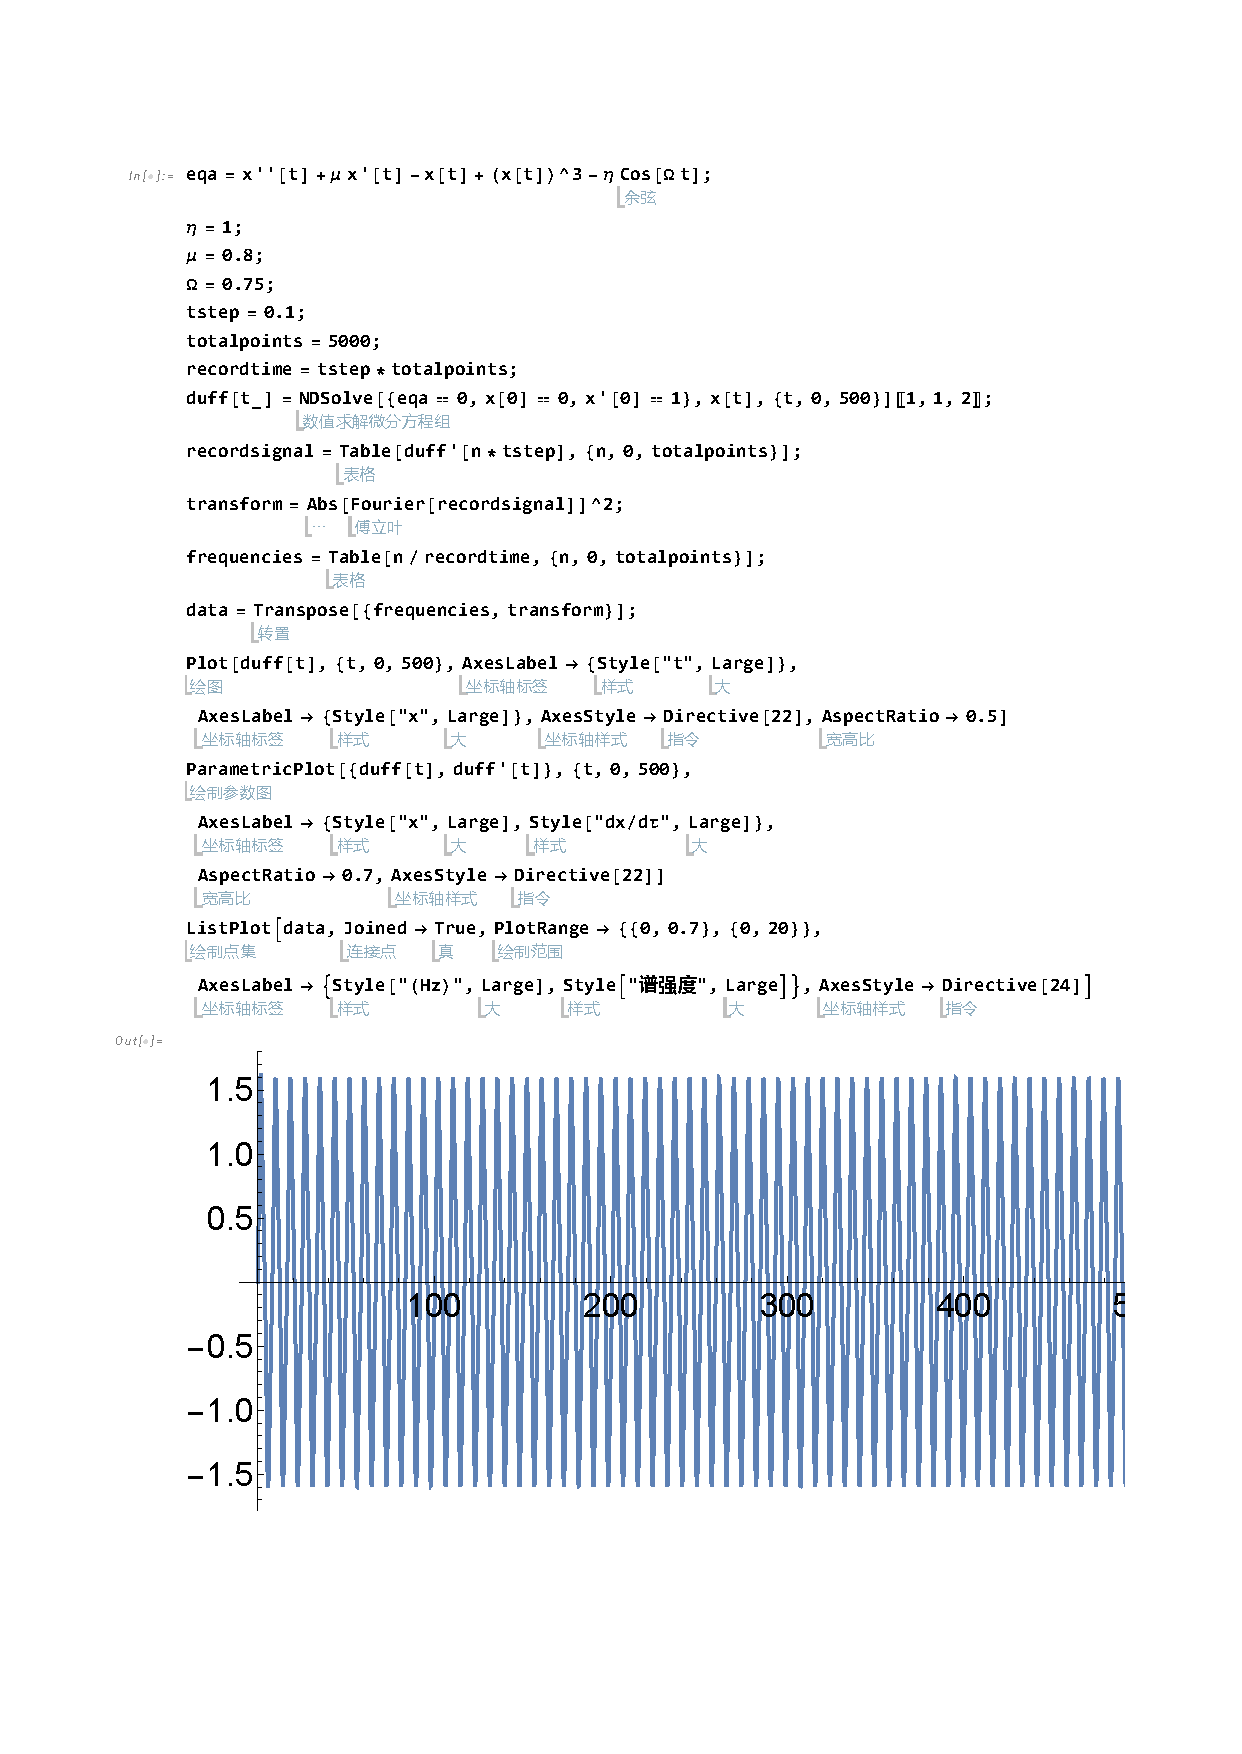
\includepdf[pages=-]{chaos.pdf}
\subsection*{原件扫描}
\includepdf[pages=-]{实验4原件.pdf}

\subsection*{桌面}
\begin{figure}[!h]
	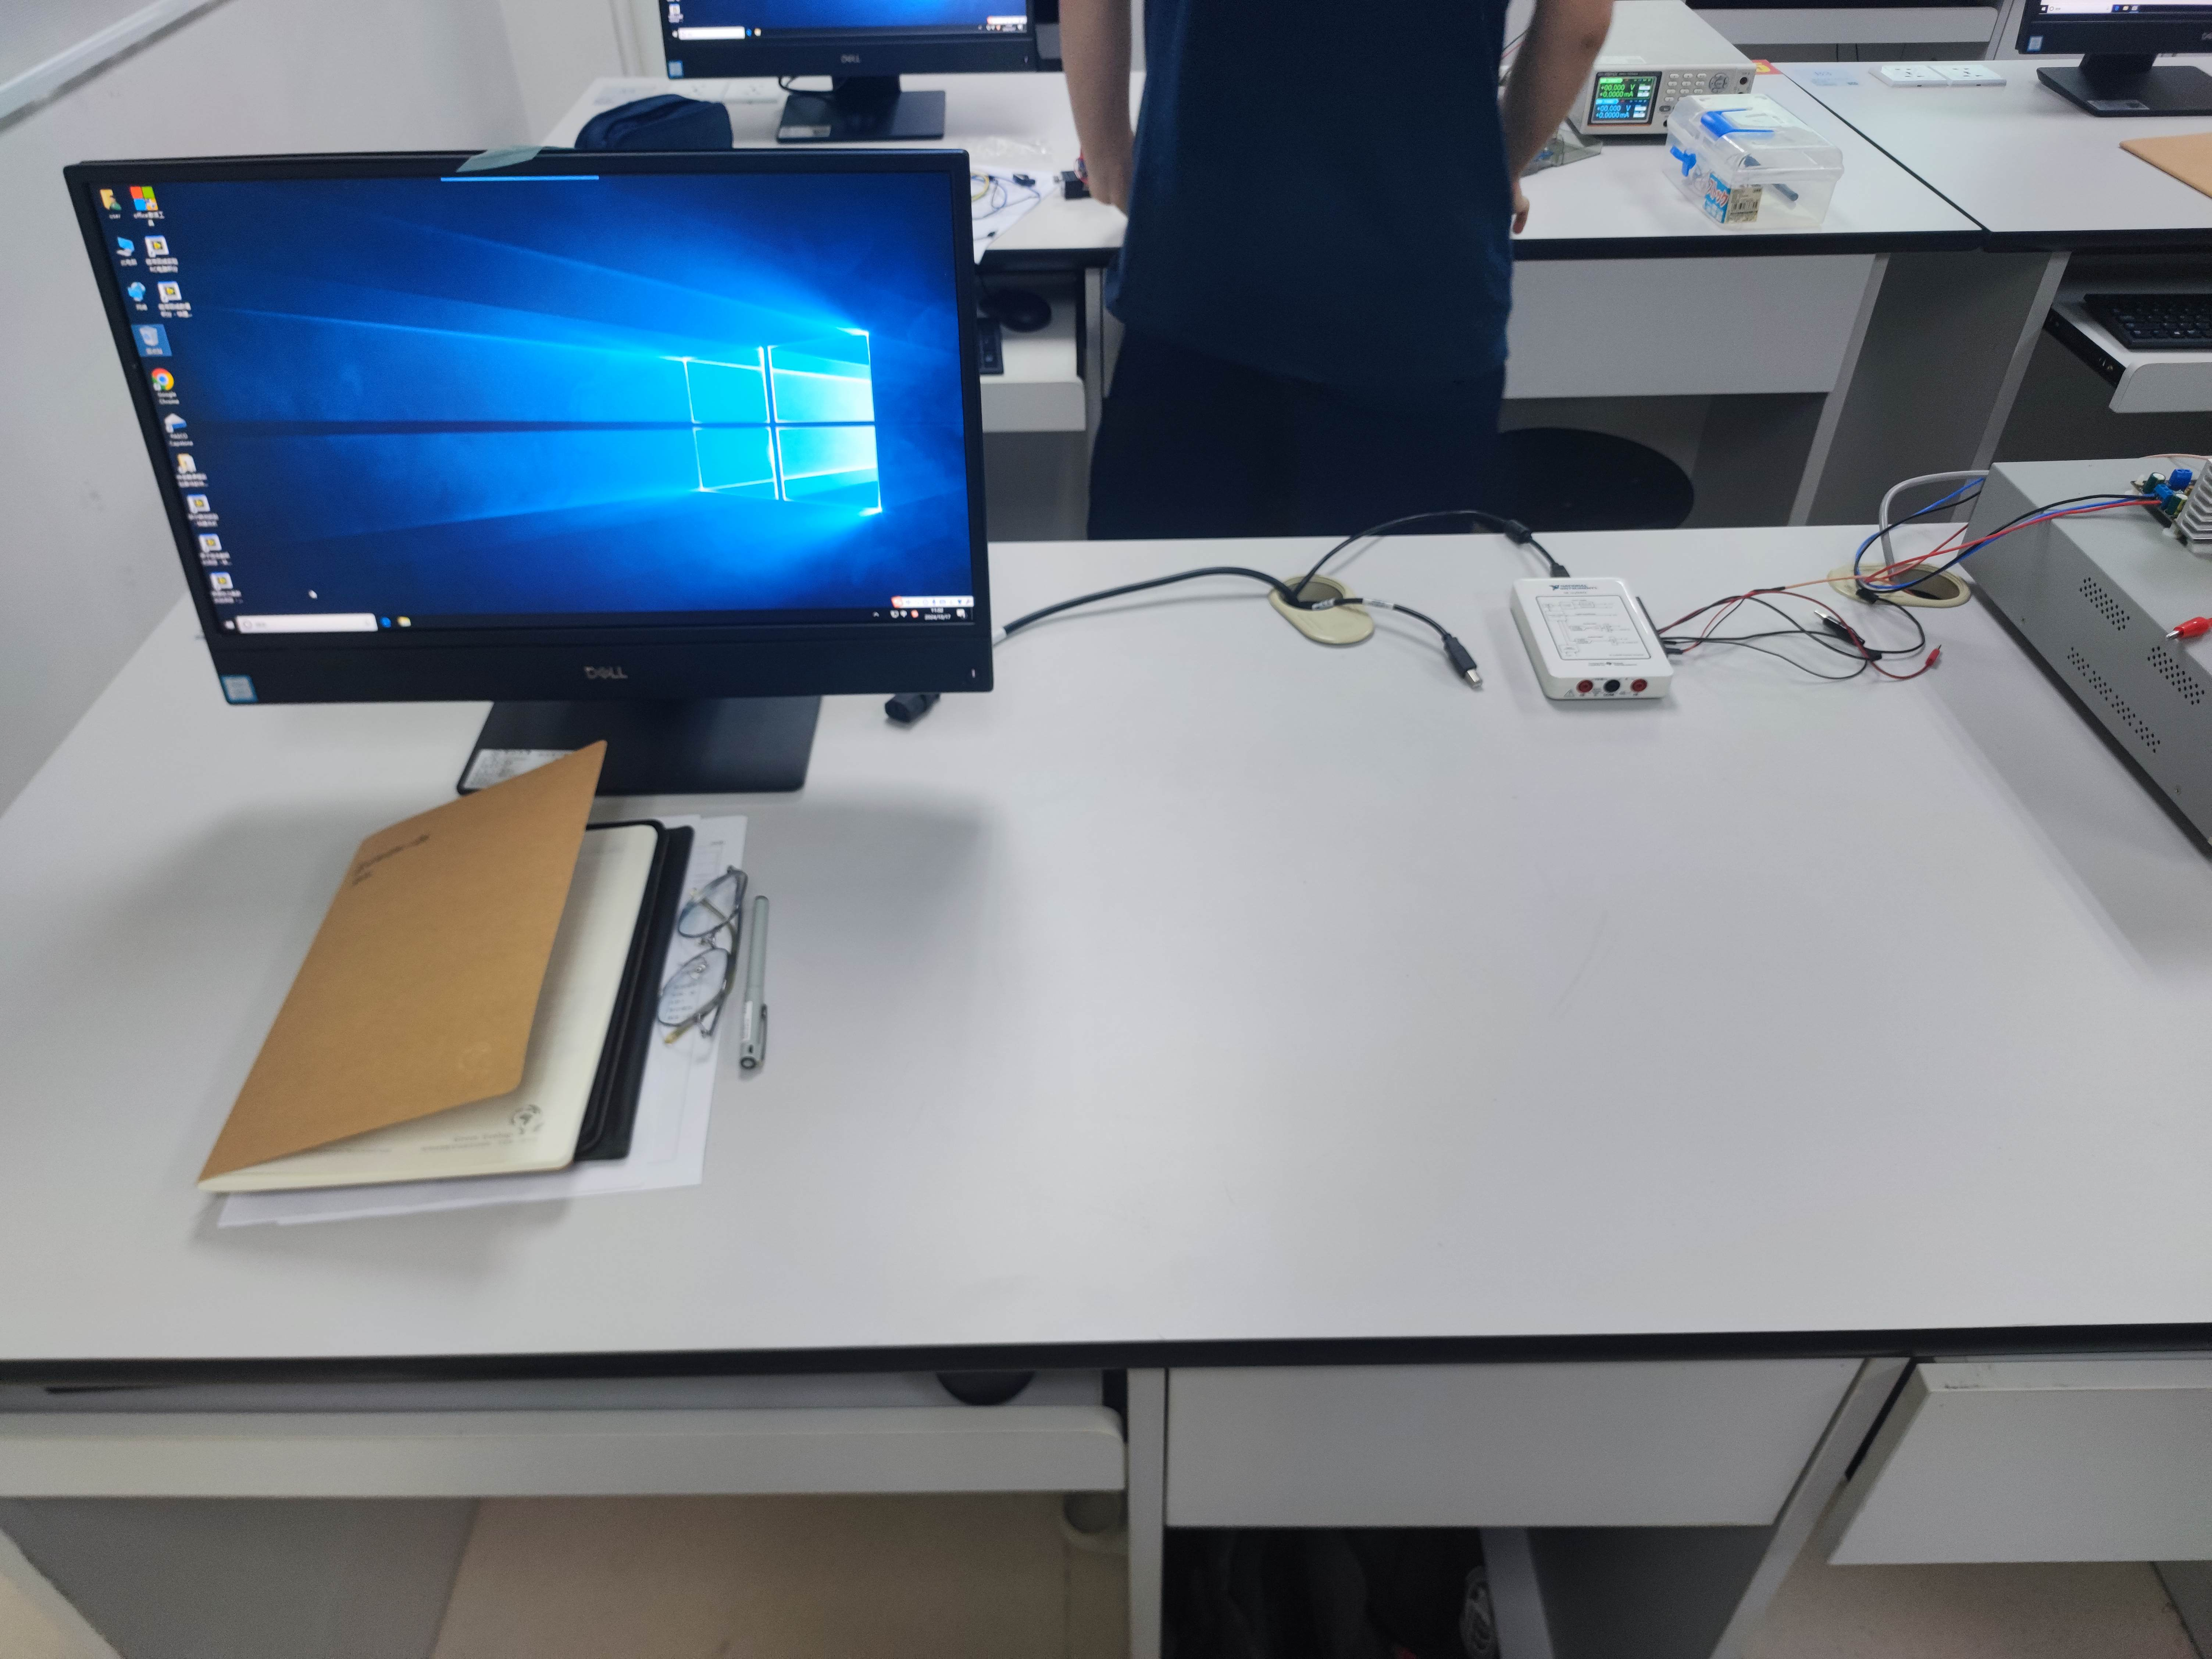
\includegraphics[width=0.95\textwidth]{实验4桌面.jpg}
\end{figure}
\end{document}